\documentclass[1p]{elsarticle_modified}
%\bibliographystyle{elsarticle-num}

%\usepackage[colorlinks]{hyperref}
%\usepackage{abbrmath_seonhwa} %\Abb, \Ascr, \Acal ,\Abf, \Afrak
\usepackage{amsfonts}
\usepackage{amssymb}
\usepackage{amsmath}
\usepackage{amsthm}
\usepackage{scalefnt}
\usepackage{amsbsy}
\usepackage{kotex}
\usepackage{caption}
\usepackage{subfig}
\usepackage{color}
\usepackage{graphicx}
\usepackage{xcolor} %% white, black, red, green, blue, cyan, magenta, yellow
\usepackage{float}
\usepackage{setspace}
\usepackage{hyperref}

\usepackage{tikz}
\usetikzlibrary{arrows}

\usepackage{multirow}
\usepackage{array} % fixed length table
\usepackage{hhline}

%%%%%%%%%%%%%%%%%%%%%
\makeatletter
\renewcommand*\env@matrix[1][\arraystretch]{%
	\edef\arraystretch{#1}%
	\hskip -\arraycolsep
	\let\@ifnextchar\new@ifnextchar
	\array{*\c@MaxMatrixCols c}}
\makeatother %https://tex.stackexchange.com/questions/14071/how-can-i-increase-the-line-spacing-in-a-matrix
%%%%%%%%%%%%%%%

\usepackage[normalem]{ulem}

\newcommand{\msout}[1]{\ifmmode\text{\sout{\ensuremath{#1}}}\else\sout{#1}\fi}
%SOURCE: \msout is \stkout macro in https://tex.stackexchange.com/questions/20609/strikeout-in-math-mode

\newcommand{\cancel}[1]{
	\ifmmode
	{\color{red}\msout{#1}}
	\else
	{\color{red}\sout{#1}}
	\fi
}

\newcommand{\add}[1]{
	{\color{blue}\uwave{#1}}
}

\newcommand{\replace}[2]{
	\ifmmode
	{\color{red}\msout{#1}}{\color{blue}\uwave{#2}}
	\else
	{\color{red}\sout{#1}}{\color{blue}\uwave{#2}}
	\fi
}

\newcommand{\Sol}{\mathcal{S}} %segment
\newcommand{\D}{D} %diagram
\newcommand{\A}{\mathcal{A}} %arc


%%%%%%%%%%%%%%%%%%%%%%%%%%%%%5 test

\def\sl{\operatorname{\textup{SL}}(2,\Cbb)}
\def\psl{\operatorname{\textup{PSL}}(2,\Cbb)}
\def\quan{\mkern 1mu \triangleright \mkern 1mu}

\theoremstyle{definition}
\newtheorem{thm}{Theorem}[section]
\newtheorem{prop}[thm]{Proposition}
\newtheorem{lem}[thm]{Lemma}
\newtheorem{ques}[thm]{Question}
\newtheorem{cor}[thm]{Corollary}
\newtheorem{defn}[thm]{Definition}
\newtheorem{exam}[thm]{Example}
\newtheorem{rmk}[thm]{Remark}
\newtheorem{alg}[thm]{Algorithm}

\newcommand{\I}{\sqrt{-1}}
\begin{document}

%\begin{frontmatter}
%
%\title{Boundary parabolic representations of knots up to 8 crossings}
%
%%% Group authors per affiliation:
%\author{Yunhi Cho} 
%\address{Department of Mathematics, University of Seoul, Seoul, Korea}
%\ead{yhcho@uos.ac.kr}
%
%
%\author{Seonhwa Kim} %\fnref{s_kim}}
%\address{Center for Geometry and Physics, Institute for Basic Science, Pohang, 37673, Korea}
%\ead{ryeona17@ibs.re.kr}
%
%\author{Hyuk Kim}
%\address{Department of Mathematical Sciences, Seoul National University, Seoul 08826, Korea}
%\ead{hyukkim@snu.ac.kr}
%
%\author{Seokbeom Yoon}
%\address{Department of Mathematical Sciences, Seoul National University, Seoul, 08826,  Korea}
%\ead{sbyoon15@snu.ac.kr}
%
%\begin{abstract}
%We find all boundary parabolic representation of knots up to 8 crossings.
%
%\end{abstract}
%\begin{keyword}
%    \MSC[2010] 57M25 
%\end{keyword}
%
%\end{frontmatter}

%\linenumbers
%\tableofcontents
%
\newcommand\colored[1]{\textcolor{white}{\rule[-0.35ex]{0.8em}{1.4ex}}\kern-0.8em\color{red} #1}%
%\newcommand\colored[1]{\textcolor{white}{ #1}\kern-2.17ex	\textcolor{white}{ #1}\kern-1.81ex	\textcolor{white}{ #1}\kern-2.15ex\color{red}#1	}

{\Large $\underline{12a_{0497}~(K12a_{0497})}$}

\setlength{\tabcolsep}{10pt}
\renewcommand{\arraystretch}{1.6}
\vspace{1cm}\begin{tabular}{m{100pt}>{\centering\arraybackslash}m{274pt}}
\multirow{5}{120pt}{
	\centering
	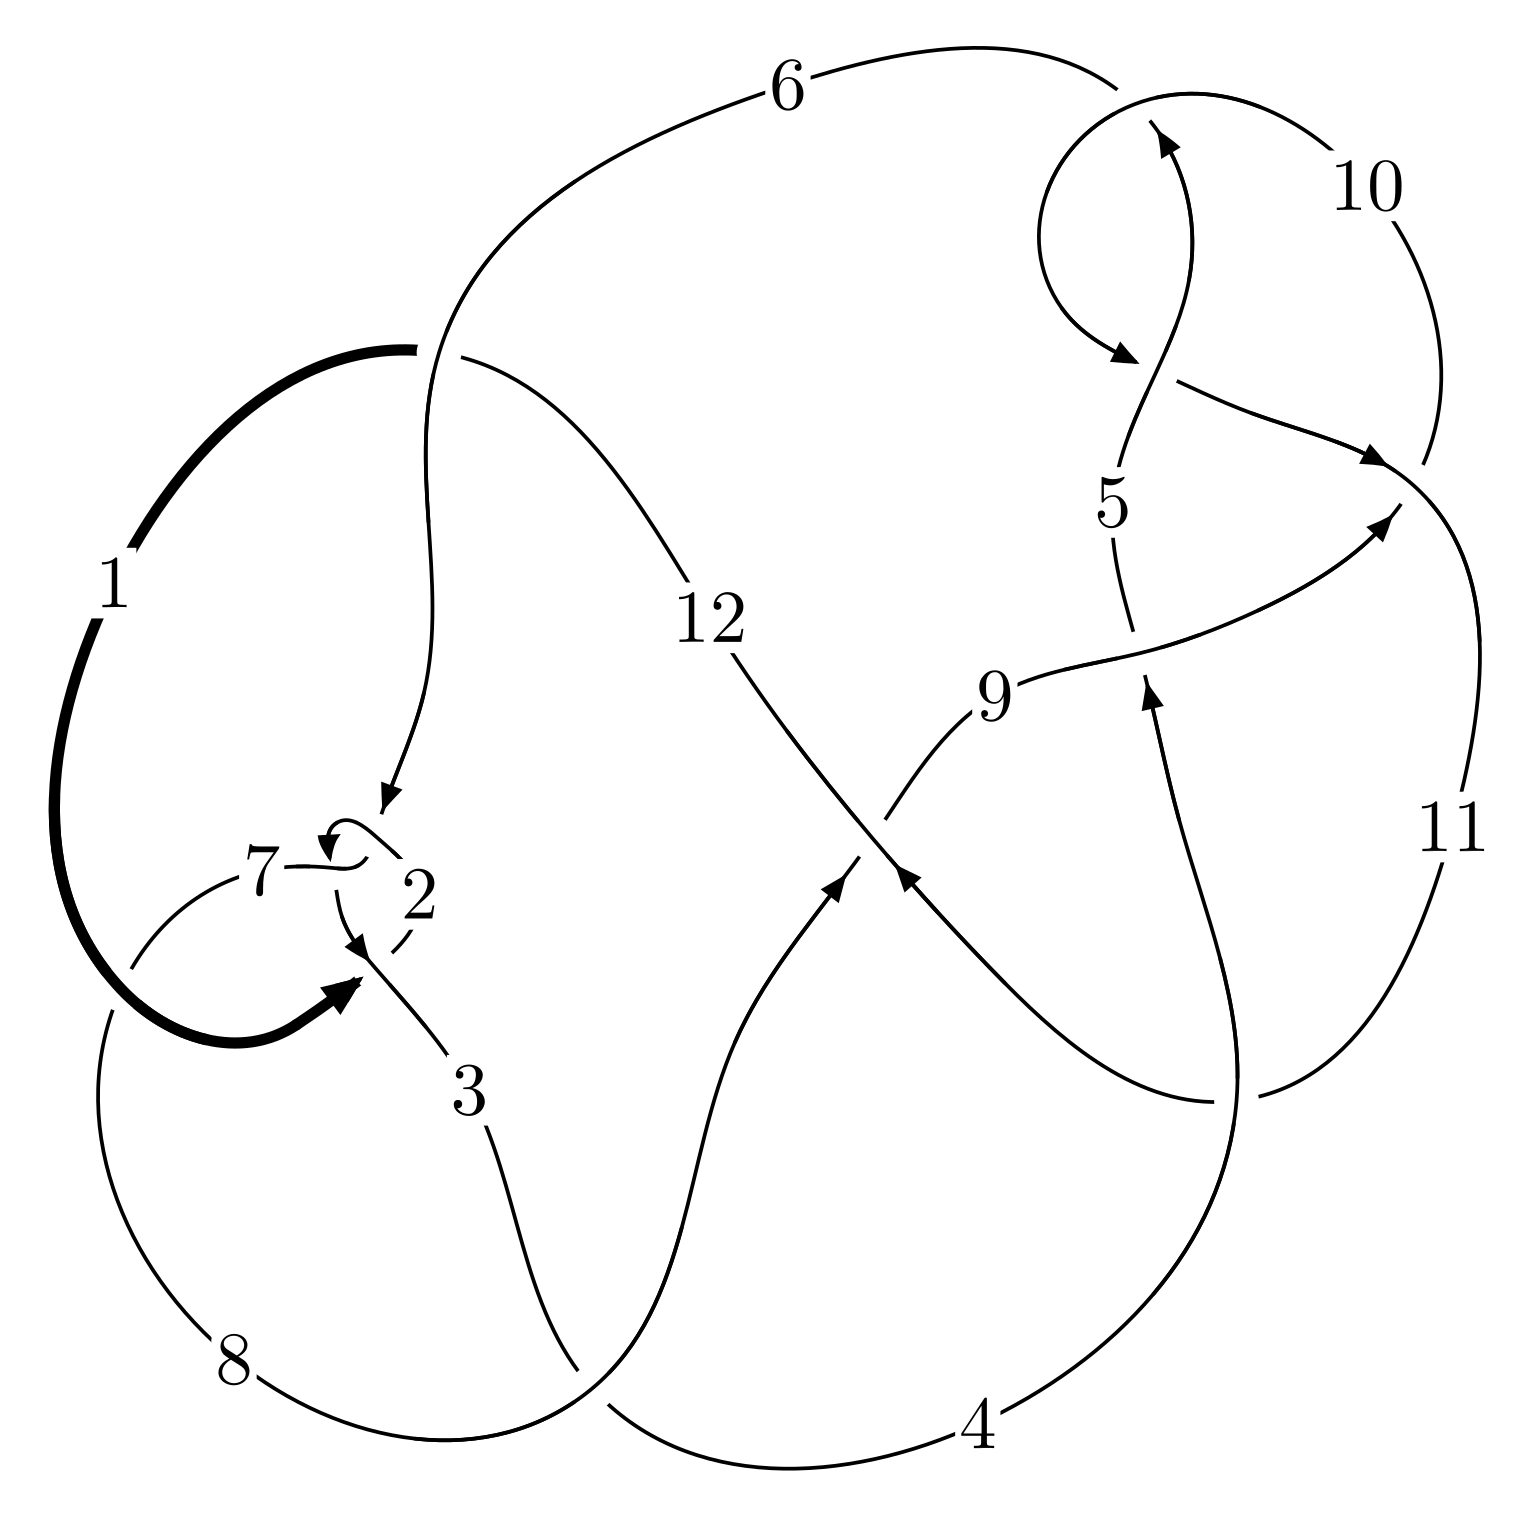
\includegraphics[width=112pt]{../../../GIT/diagram.site/Diagrams/png/1298_12a_0497.png}\\
\ \ \ A knot diagram\footnotemark}&
\allowdisplaybreaks
\textbf{Linearized knot diagam} \\
\cline{2-2}
 &
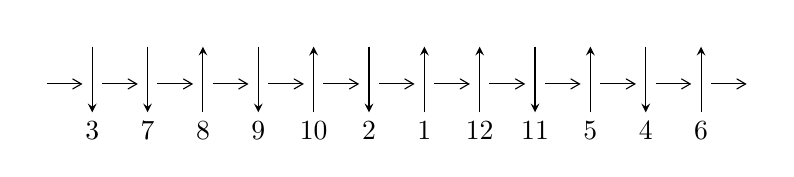
\begin{tikzpicture}[x=20pt, y=17pt]
	% nodes
	\node (C0) at (0, 0) {};
	\node (C1) at (1, 0) {};
	\node (C1U) at (1, +1) {};
	\node (C1D) at (1, -1) {3};

	\node (C2) at (2, 0) {};
	\node (C2U) at (2, +1) {};
	\node (C2D) at (2, -1) {7};

	\node (C3) at (3, 0) {};
	\node (C3U) at (3, +1) {};
	\node (C3D) at (3, -1) {8};

	\node (C4) at (4, 0) {};
	\node (C4U) at (4, +1) {};
	\node (C4D) at (4, -1) {9};

	\node (C5) at (5, 0) {};
	\node (C5U) at (5, +1) {};
	\node (C5D) at (5, -1) {10};

	\node (C6) at (6, 0) {};
	\node (C6U) at (6, +1) {};
	\node (C6D) at (6, -1) {2};

	\node (C7) at (7, 0) {};
	\node (C7U) at (7, +1) {};
	\node (C7D) at (7, -1) {1};

	\node (C8) at (8, 0) {};
	\node (C8U) at (8, +1) {};
	\node (C8D) at (8, -1) {12};

	\node (C9) at (9, 0) {};
	\node (C9U) at (9, +1) {};
	\node (C9D) at (9, -1) {11};

	\node (C10) at (10, 0) {};
	\node (C10U) at (10, +1) {};
	\node (C10D) at (10, -1) {5};

	\node (C11) at (11, 0) {};
	\node (C11U) at (11, +1) {};
	\node (C11D) at (11, -1) {4};

	\node (C12) at (12, 0) {};
	\node (C12U) at (12, +1) {};
	\node (C12D) at (12, -1) {6};
	\node (C13) at (13, 0) {};

	% arrows
	\draw[->,>={angle 60}]
	(C0) edge (C1) (C1) edge (C2) (C2) edge (C3) (C3) edge (C4) (C4) edge (C5) (C5) edge (C6) (C6) edge (C7) (C7) edge (C8) (C8) edge (C9) (C9) edge (C10) (C10) edge (C11) (C11) edge (C12) (C12) edge (C13) ;	\draw[->,>=stealth]
	(C1U) edge (C1D) (C2U) edge (C2D) (C3D) edge (C3U) (C4U) edge (C4D) (C5D) edge (C5U) (C6U) edge (C6D) (C7D) edge (C7U) (C8D) edge (C8U) (C9U) edge (C9D) (C10D) edge (C10U) (C11U) edge (C11D) (C12D) edge (C12U) ;
	\end{tikzpicture} \\
\hhline{~~} \\& 
\textbf{Solving Sequence} \\ \cline{2-2} 
 &
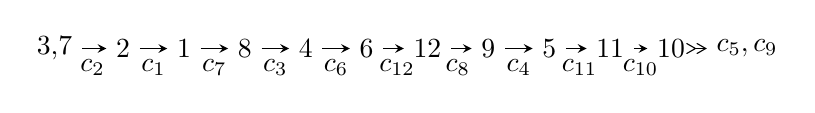
\begin{tikzpicture}[x=22pt, y=7pt]
	% node
	\node (A0) at (-1/8, 0) {3,7};
	\node (A1) at (1, 0) {2};
	\node (A2) at (2, 0) {1};
	\node (A3) at (3, 0) {8};
	\node (A4) at (4, 0) {4};
	\node (A5) at (5, 0) {6};
	\node (A6) at (6, 0) {12};
	\node (A7) at (7, 0) {9};
	\node (A8) at (8, 0) {5};
	\node (A9) at (9, 0) {11};
	\node (A10) at (10, 0) {10};
	\node (C1) at (1/2, -1) {$c_{2}$};
	\node (C2) at (3/2, -1) {$c_{1}$};
	\node (C3) at (5/2, -1) {$c_{7}$};
	\node (C4) at (7/2, -1) {$c_{3}$};
	\node (C5) at (9/2, -1) {$c_{6}$};
	\node (C6) at (11/2, -1) {$c_{12}$};
	\node (C7) at (13/2, -1) {$c_{8}$};
	\node (C8) at (15/2, -1) {$c_{4}$};
	\node (C9) at (17/2, -1) {$c_{11}$};
	\node (C10) at (19/2, -1) {$c_{10}$};
	\node (A11) at (45/4, 0) {$c_{5},c_{9}$};

	% edge
	\draw[->,>=stealth]	
	(A0) edge (A1) (A1) edge (A2) (A2) edge (A3) (A3) edge (A4) (A4) edge (A5) (A5) edge (A6) (A6) edge (A7) (A7) edge (A8) (A8) edge (A9) (A9) edge (A10) ;
	\draw[->>,>={angle 60}]	
	(A10) edge (A11);
\end{tikzpicture} \\ 

\end{tabular} \\

\footnotetext{
The image of knot diagram is generated by the software ``\textbf{Draw programme}" developed by Andrew Bartholomew(\url{http://www.layer8.co.uk/maths/draw/index.htm\#Running-draw}), where we modified some parts for our purpose(\url{https://github.com/CATsTAILs/LinksPainter}).
}\phantom \\ \newline 
\centering \textbf{Ideals for irreducible components\footnotemark of $X_{\text{par}}$} 
 
\begin{align*}
I^u_{1}&=\langle 
u^{104}- u^{103}+\cdots+2 u^3+1\rangle \\
\\
\end{align*}
\raggedright * 1 irreducible components of $\dim_{\mathbb{C}}=0$, with total 104 representations.\\
\footnotetext{All coefficients of polynomials are rational numbers. But the coefficients are sometimes approximated in decimal forms when there is not enough margin.}
\newpage
\renewcommand{\arraystretch}{1}
\centering \section*{I. $I^u_{1}= \langle u^{104}- u^{103}+\cdots+2 u^3+1 \rangle$}
\flushleft \textbf{(i) Arc colorings}\\
\begin{tabular}{m{7pt} m{180pt} m{7pt} m{180pt} }
\flushright $a_{3}=$&$\begin{pmatrix}1\\0\end{pmatrix}$ \\
\flushright $a_{7}=$&$\begin{pmatrix}0\\u\end{pmatrix}$ \\
\flushright $a_{2}=$&$\begin{pmatrix}1\\- u^2\end{pmatrix}$ \\
\flushright $a_{1}=$&$\begin{pmatrix}- u^2+1\\- u^2\end{pmatrix}$ \\
\flushright $a_{8}=$&$\begin{pmatrix}u^5-2 u^3+u\\u^5- u^3+u\end{pmatrix}$ \\
\flushright $a_{4}=$&$\begin{pmatrix}- u^{10}+3 u^8-4 u^6+3 u^4- u^2+1\\- u^{10}+2 u^8-3 u^6+2 u^4- u^2\end{pmatrix}$ \\
\flushright $a_{6}=$&$\begin{pmatrix}u\\- u^3+u\end{pmatrix}$ \\
\flushright $a_{12}=$&$\begin{pmatrix}u^6- u^4+1\\- u^8+2 u^6-2 u^4\end{pmatrix}$ \\
\flushright $a_{9}=$&$\begin{pmatrix}u^{19}-4 u^{17}+8 u^{15}-8 u^{13}+3 u^{11}+2 u^9-2 u^7+2 u^5-3 u^3+2 u\\- u^{21}+5 u^{19}-13 u^{17}+20 u^{15}-20 u^{13}+13 u^{11}-7 u^9+4 u^7- u^5- u^3+u\end{pmatrix}$ \\
\flushright $a_{5}=$&$\begin{pmatrix}u^{50}-11 u^{48}+\cdots+u^2+1\\- u^{52}+12 u^{50}+\cdots-8 u^6+u^4\end{pmatrix}$ \\
\flushright $a_{11}=$&$\begin{pmatrix}- u^{28}+7 u^{26}+\cdots+u^2+1\\- u^{28}+6 u^{26}+\cdots+8 u^6-3 u^4\end{pmatrix}$ \\
\flushright $a_{10}=$&$\begin{pmatrix}u^{77}-18 u^{75}+\cdots-4 u^3+u\\u^{77}-17 u^{75}+\cdots- u^3+u\end{pmatrix}$\\&\end{tabular}
\flushleft \textbf{(ii) Obstruction class $= -1$}\\~\\
\flushleft \textbf{(iii) Cusp Shapes $= 4 u^{102}-92 u^{100}+\cdots-4 u^2-2$}\\~\\
\newpage\renewcommand{\arraystretch}{1}
\flushleft \textbf{(iv) u-Polynomials at the component}\newline \\
\begin{tabular}{m{50pt}|m{274pt}}
Crossings & \hspace{64pt}u-Polynomials at each crossing \\
\hline $$\begin{aligned}c_{1}\end{aligned}$$&$\begin{aligned}
&u^{104}+47 u^{103}+\cdots+2 u^2+1
\end{aligned}$\\
\hline $$\begin{aligned}c_{2},c_{6}\end{aligned}$$&$\begin{aligned}
&u^{104}- u^{103}+\cdots+2 u^3+1
\end{aligned}$\\
\hline $$\begin{aligned}c_{3},c_{12}\end{aligned}$$&$\begin{aligned}
&u^{104}+u^{103}+\cdots-22 u+1
\end{aligned}$\\
\hline $$\begin{aligned}c_{4}\end{aligned}$$&$\begin{aligned}
&u^{104}- u^{103}+\cdots-4786 u+1237
\end{aligned}$\\
\hline $$\begin{aligned}c_{5},c_{10}\end{aligned}$$&$\begin{aligned}
&u^{104}+u^{103}+\cdots+2 u+1
\end{aligned}$\\
\hline $$\begin{aligned}c_{7}\end{aligned}$$&$\begin{aligned}
&u^{104}-3 u^{103}+\cdots-8 u+3
\end{aligned}$\\
\hline $$\begin{aligned}c_{8}\end{aligned}$$&$\begin{aligned}
&u^{104}+13 u^{103}+\cdots+20 u+1
\end{aligned}$\\
\hline $$\begin{aligned}c_{9}\end{aligned}$$&$\begin{aligned}
&u^{104}+49 u^{103}+\cdots+2 u^2+1
\end{aligned}$\\
\hline $$\begin{aligned}c_{11}\end{aligned}$$&$\begin{aligned}
&u^{104}+5 u^{103}+\cdots+17926 u+3477
\end{aligned}$\\
\hline
\end{tabular}\\~\\
\newpage\renewcommand{\arraystretch}{1}
\flushleft \textbf{(v) Riley Polynomials at the component}\newline \\
\begin{tabular}{m{50pt}|m{274pt}}
Crossings & \hspace{64pt}Riley Polynomials at each crossing \\
\hline $$\begin{aligned}c_{1}\end{aligned}$$&$\begin{aligned}
&y^{104}+21 y^{103}+\cdots+4 y+1
\end{aligned}$\\
\hline $$\begin{aligned}c_{2},c_{6}\end{aligned}$$&$\begin{aligned}
&y^{104}-47 y^{103}+\cdots+2 y^2+1
\end{aligned}$\\
\hline $$\begin{aligned}c_{3},c_{12}\end{aligned}$$&$\begin{aligned}
&y^{104}-79 y^{103}+\cdots+112 y+1
\end{aligned}$\\
\hline $$\begin{aligned}c_{4}\end{aligned}$$&$\begin{aligned}
&y^{104}-23 y^{103}+\cdots-66086992 y+1530169
\end{aligned}$\\
\hline $$\begin{aligned}c_{5},c_{10}\end{aligned}$$&$\begin{aligned}
&y^{104}+49 y^{103}+\cdots+2 y^2+1
\end{aligned}$\\
\hline $$\begin{aligned}c_{7}\end{aligned}$$&$\begin{aligned}
&y^{104}+5 y^{103}+\cdots+800 y+9
\end{aligned}$\\
\hline $$\begin{aligned}c_{8}\end{aligned}$$&$\begin{aligned}
&y^{104}+y^{103}+\cdots+284 y+1
\end{aligned}$\\
\hline $$\begin{aligned}c_{9}\end{aligned}$$&$\begin{aligned}
&y^{104}+13 y^{103}+\cdots+4 y+1
\end{aligned}$\\
\hline $$\begin{aligned}c_{11}\end{aligned}$$&$\begin{aligned}
&y^{104}+29 y^{103}+\cdots+539591540 y+12089529
\end{aligned}$\\
\hline
\end{tabular}\\~\\
\newpage\flushleft \textbf{(vi) Complex Volumes and Cusp Shapes}
$$\begin{array}{c|c|c}  
\text{Solutions to }I^u_{1}& \I (\text{vol} + \sqrt{-1}CS) & \text{Cusp shape}\\
 \hline 
\begin{aligned}
u &= -0.859307 + 0.524203 I\end{aligned}
 & -0.01758 + 7.72337 I & \phantom{-0.000000 } 0 \\ \hline\begin{aligned}
u &= -0.859307 - 0.524203 I\end{aligned}
 & -0.01758 - 7.72337 I & \phantom{-0.000000 } 0 \\ \hline\begin{aligned}
u &= \phantom{-}0.836775 + 0.503199 I\end{aligned}
 & \phantom{-}1.90773 - 2.97029 I & \phantom{-0.000000 } 0 \\ \hline\begin{aligned}
u &= \phantom{-}0.836775 - 0.503199 I\end{aligned}
 & \phantom{-}1.90773 + 2.97029 I & \phantom{-0.000000 } 0 \\ \hline\begin{aligned}
u &= -1.011650 + 0.233039 I\end{aligned}
 & -2.04169 + 0.66017 I & \phantom{-0.000000 } 0 \\ \hline\begin{aligned}
u &= -1.011650 - 0.233039 I\end{aligned}
 & -2.04169 - 0.66017 I & \phantom{-0.000000 } 0 \\ \hline\begin{aligned}
u &= -0.980187 + 0.397197 I\end{aligned}
 & -1.88622 + 1.31284 I & \phantom{-0.000000 } 0 \\ \hline\begin{aligned}
u &= -0.980187 - 0.397197 I\end{aligned}
 & -1.88622 - 1.31284 I & \phantom{-0.000000 } 0 \\ \hline\begin{aligned}
u &= -1.056710 + 0.066632 I\end{aligned}
 & \phantom{-}0.57803 + 2.08421 I & \phantom{-0.000000 } 0 \\ \hline\begin{aligned}
u &= -1.056710 - 0.066632 I\end{aligned}
 & \phantom{-}0.57803 - 2.08421 I & \phantom{-0.000000 } 0 \\ \hline\begin{aligned}
u &= -0.958501 + 0.452296 I\end{aligned}
 & -1.91153 + 1.29780 I & \phantom{-0.000000 } 0 \\ \hline\begin{aligned}
u &= -0.958501 - 0.452296 I\end{aligned}
 & -1.91153 - 1.29780 I & \phantom{-0.000000 } 0 \\ \hline\begin{aligned}
u &= \phantom{-}1.070350 + 0.091384 I\end{aligned}
 & \phantom{-}1.69880 + 2.66563 I & \phantom{-0.000000 } 0 \\ \hline\begin{aligned}
u &= \phantom{-}1.070350 - 0.091384 I\end{aligned}
 & \phantom{-}1.69880 - 2.66563 I & \phantom{-0.000000 } 0 \\ \hline\begin{aligned}
u &= \phantom{-}1.055850 + 0.204960 I\end{aligned}
 & -5.41329 + 2.54049 I & \phantom{-0.000000 } 0 \\ \hline\begin{aligned}
u &= \phantom{-}1.055850 - 0.204960 I\end{aligned}
 & -5.41329 - 2.54049 I & \phantom{-0.000000 } 0 \\ \hline\begin{aligned}
u &= \phantom{-}0.542072 + 0.741306 I\end{aligned}
 & \phantom{-}3.99783 - 9.10436 I & \phantom{-0.000000 } 0 \\ \hline\begin{aligned}
u &= \phantom{-}0.542072 - 0.741306 I\end{aligned}
 & \phantom{-}3.99783 + 9.10436 I & \phantom{-0.000000 } 0 \\ \hline\begin{aligned}
u &= \phantom{-}1.051860 + 0.253380 I\end{aligned}
 & -4.49361 - 4.87932 I & \phantom{-0.000000 } 0 \\ \hline\begin{aligned}
u &= \phantom{-}1.051860 - 0.253380 I\end{aligned}
 & -4.49361 + 4.87932 I & \phantom{-0.000000 } 0 \\ \hline\begin{aligned}
u &= -0.534590 + 0.741284 I\end{aligned}
 & \phantom{-}6.16977 + 4.04816 I & \phantom{-0.000000 } 0 \\ \hline\begin{aligned}
u &= -0.534590 - 0.741284 I\end{aligned}
 & \phantom{-}6.16977 - 4.04816 I & \phantom{-0.000000 } 0 \\ \hline\begin{aligned}
u &= -0.515131 + 0.748064 I\end{aligned}
 & \phantom{-}7.20284 + 1.69792 I & \phantom{-0.000000 } 0 \\ \hline\begin{aligned}
u &= -0.515131 - 0.748064 I\end{aligned}
 & \phantom{-}7.20284 - 1.69792 I & \phantom{-0.000000 } 0 \\ \hline\begin{aligned}
u &= -1.083390 + 0.136794 I\end{aligned}
 & -4.04015 - 2.23636 I & \phantom{-0.000000 } 0 \\ \hline\begin{aligned}
u &= -1.083390 - 0.136794 I\end{aligned}
 & -4.04015 + 2.23636 I & \phantom{-0.000000 } 0 \\ \hline\begin{aligned}
u &= \phantom{-}0.504216 + 0.753178 I\end{aligned}
 & \phantom{-}5.99912 + 3.19718 I & \phantom{-0.000000 } 0 \\ \hline\begin{aligned}
u &= \phantom{-}0.504216 - 0.753178 I\end{aligned}
 & \phantom{-}5.99912 - 3.19718 I & \phantom{-0.000000 } 0 \\ \hline\begin{aligned}
u &= \phantom{-}1.092950 + 0.116654 I\end{aligned}
 & \phantom{-}0.50313 + 4.81762 I & \phantom{-0.000000 } 0 \\ \hline\begin{aligned}
u &= \phantom{-}1.092950 - 0.116654 I\end{aligned}
 & \phantom{-}0.50313 - 4.81762 I & \phantom{-0.000000 } 0\\
 \hline 
 \end{array}$$\newpage$$\begin{array}{c|c|c}  
\text{Solutions to }I^u_{1}& \I (\text{vol} + \sqrt{-1}CS) & \text{Cusp shape}\\
 \hline 
\begin{aligned}
u &= \phantom{-}0.756728 + 0.484409 I\end{aligned}
 & \phantom{-}2.14268 - 1.17121 I & \phantom{-}6.64343 + 0. I\phantom{ +0.000000I} \\ \hline\begin{aligned}
u &= \phantom{-}0.756728 - 0.484409 I\end{aligned}
 & \phantom{-}2.14268 + 1.17121 I & \phantom{-}6.64343 + 0. I\phantom{ +0.000000I} \\ \hline\begin{aligned}
u &= \phantom{-}0.531824 + 0.723039 I\end{aligned}
 & \phantom{-}1.51039 - 1.63841 I & \phantom{-0.000000 } 0 \\ \hline\begin{aligned}
u &= \phantom{-}0.531824 - 0.723039 I\end{aligned}
 & \phantom{-}1.51039 + 1.63841 I & \phantom{-0.000000 } 0 \\ \hline\begin{aligned}
u &= \phantom{-}0.453000 + 0.771117 I\end{aligned}
 & \phantom{-}5.72060 - 0.33111 I & \phantom{-}5.65604 + 0. I\phantom{ +0.000000I} \\ \hline\begin{aligned}
u &= \phantom{-}0.453000 - 0.771117 I\end{aligned}
 & \phantom{-}5.72060 + 0.33111 I & \phantom{-}5.65604 + 0. I\phantom{ +0.000000I} \\ \hline\begin{aligned}
u &= -0.442763 + 0.774845 I\end{aligned}
 & \phantom{-}6.80677 - 4.55207 I & \phantom{-}7.37432 + 3.79202 I \\ \hline\begin{aligned}
u &= -0.442763 - 0.774845 I\end{aligned}
 & \phantom{-}6.80677 + 4.55207 I & \phantom{-}7.37432 - 3.79202 I \\ \hline\begin{aligned}
u &= -1.101690 + 0.121004 I\end{aligned}
 & -1.74425 - 9.83174 I & \phantom{-0.000000 } 0 \\ \hline\begin{aligned}
u &= -1.101690 - 0.121004 I\end{aligned}
 & -1.74425 + 9.83174 I & \phantom{-0.000000 } 0 \\ \hline\begin{aligned}
u &= \phantom{-}0.422973 + 0.784494 I\end{aligned}
 & \phantom{-}3.34574 + 11.96320 I & \phantom{-0.000000 } 0. - 7.58874 I \\ \hline\begin{aligned}
u &= \phantom{-}0.422973 - 0.784494 I\end{aligned}
 & \phantom{-}3.34574 - 11.96320 I & \phantom{-0.000000 -}0. + 7.58874 I \\ \hline\begin{aligned}
u &= -0.427276 + 0.781006 I\end{aligned}
 & \phantom{-}5.58256 - 6.89102 I & \phantom{-}5.88164 + 3.70083 I \\ \hline\begin{aligned}
u &= -0.427276 - 0.781006 I\end{aligned}
 & \phantom{-}5.58256 + 6.89102 I & \phantom{-}5.88164 - 3.70083 I \\ \hline\begin{aligned}
u &= \phantom{-}0.420575 + 0.770410 I\end{aligned}
 & \phantom{-}0.90649 + 4.32693 I & \phantom{-0.000000 } 0. - 2.33566 I \\ \hline\begin{aligned}
u &= \phantom{-}0.420575 - 0.770410 I\end{aligned}
 & \phantom{-}0.90649 - 4.32693 I & \phantom{-0.000000 -}0. + 2.33566 I \\ \hline\begin{aligned}
u &= -0.705886 + 0.507842 I\end{aligned}
 & \phantom{-}0.40911 - 3.44910 I & \phantom{-}3.11069 + 2.13802 I \\ \hline\begin{aligned}
u &= -0.705886 - 0.507842 I\end{aligned}
 & \phantom{-}0.40911 + 3.44910 I & \phantom{-}3.11069 - 2.13802 I \\ \hline\begin{aligned}
u &= -1.077900 + 0.384069 I\end{aligned}
 & -3.24714 + 0.72316 I & \phantom{-0.000000 } 0 \\ \hline\begin{aligned}
u &= -1.077900 - 0.384069 I\end{aligned}
 & -3.24714 - 0.72316 I & \phantom{-0.000000 } 0 \\ \hline\begin{aligned}
u &= \phantom{-}1.091470 + 0.378875 I\end{aligned}
 & -5.64601 + 3.93267 I & \phantom{-0.000000 } 0 \\ \hline\begin{aligned}
u &= \phantom{-}1.091470 - 0.378875 I\end{aligned}
 & -5.64601 - 3.93267 I & \phantom{-0.000000 } 0 \\ \hline\begin{aligned}
u &= \phantom{-}1.057270 + 0.468756 I\end{aligned}
 & -1.30857 - 5.15318 I & \phantom{-0.000000 } 0 \\ \hline\begin{aligned}
u &= \phantom{-}1.057270 - 0.468756 I\end{aligned}
 & -1.30857 + 5.15318 I & \phantom{-0.000000 } 0 \\ \hline\begin{aligned}
u &= \phantom{-}1.091190 + 0.402366 I\end{aligned}
 & -7.16519 - 3.66403 I & \phantom{-0.000000 } 0 \\ \hline\begin{aligned}
u &= \phantom{-}1.091190 - 0.402366 I\end{aligned}
 & -7.16519 + 3.66403 I & \phantom{-0.000000 } 0 \\ \hline\begin{aligned}
u &= \phantom{-}0.442649 + 0.704496 I\end{aligned}
 & \phantom{-}2.18390 + 1.10352 I & \phantom{-}3.36438 - 0.54429 I \\ \hline\begin{aligned}
u &= \phantom{-}0.442649 - 0.704496 I\end{aligned}
 & \phantom{-}2.18390 - 1.10352 I & \phantom{-}3.36438 + 0.54429 I \\ \hline\begin{aligned}
u &= -0.406121 + 0.717438 I\end{aligned}
 & -0.98090 - 4.64543 I & -1.49398 + 4.59581 I \\ \hline\begin{aligned}
u &= -0.406121 - 0.717438 I\end{aligned}
 & -0.98090 + 4.64543 I & -1.49398 - 4.59581 I\\
 \hline 
 \end{array}$$\newpage$$\begin{array}{c|c|c}  
\text{Solutions to }I^u_{1}& \I (\text{vol} + \sqrt{-1}CS) & \text{Cusp shape}\\
 \hline 
\begin{aligned}
u &= -1.096760 + 0.443551 I\end{aligned}
 & -6.88645 + 3.66322 I & \phantom{-0.000000 } 0 \\ \hline\begin{aligned}
u &= -1.096760 - 0.443551 I\end{aligned}
 & -6.88645 - 3.66322 I & \phantom{-0.000000 } 0 \\ \hline\begin{aligned}
u &= \phantom{-}1.092910 + 0.459875 I\end{aligned}
 & -2.73025 - 6.49785 I & \phantom{-0.000000 } 0 \\ \hline\begin{aligned}
u &= \phantom{-}1.092910 - 0.459875 I\end{aligned}
 & -2.73025 + 6.49785 I & \phantom{-0.000000 } 0 \\ \hline\begin{aligned}
u &= -1.102030 + 0.460728 I\end{aligned}
 & -5.09595 + 11.30370 I & \phantom{-0.000000 } 0 \\ \hline\begin{aligned}
u &= -1.102030 - 0.460728 I\end{aligned}
 & -5.09595 - 11.30370 I & \phantom{-0.000000 } 0 \\ \hline\begin{aligned}
u &= \phantom{-}1.033640 + 0.601494 I\end{aligned}
 & \phantom{-}0.01999 - 3.42754 I & \phantom{-0.000000 } 0 \\ \hline\begin{aligned}
u &= \phantom{-}1.033640 - 0.601494 I\end{aligned}
 & \phantom{-}0.01999 + 3.42754 I & \phantom{-0.000000 } 0 \\ \hline\begin{aligned}
u &= \phantom{-}1.031380 + 0.616617 I\end{aligned}
 & \phantom{-}2.54297 + 3.93822 I & \phantom{-0.000000 } 0 \\ \hline\begin{aligned}
u &= \phantom{-}1.031380 - 0.616617 I\end{aligned}
 & \phantom{-}2.54297 - 3.93822 I & \phantom{-0.000000 } 0 \\ \hline\begin{aligned}
u &= -1.036210 + 0.614543 I\end{aligned}
 & \phantom{-}4.67843 + 1.11092 I & \phantom{-0.000000 } 0 \\ \hline\begin{aligned}
u &= -1.036210 - 0.614543 I\end{aligned}
 & \phantom{-}4.67843 - 1.11092 I & \phantom{-0.000000 } 0 \\ \hline\begin{aligned}
u &= -1.076910 + 0.561271 I\end{aligned}
 & -2.47407 + 2.03216 I & \phantom{-0.000000 } 0 \\ \hline\begin{aligned}
u &= -1.076910 - 0.561271 I\end{aligned}
 & -2.47407 - 2.03216 I & \phantom{-0.000000 } 0 \\ \hline\begin{aligned}
u &= -1.049530 + 0.613467 I\end{aligned}
 & \phantom{-}5.61409 + 3.47527 I & \phantom{-0.000000 } 0 \\ \hline\begin{aligned}
u &= -1.049530 - 0.613467 I\end{aligned}
 & \phantom{-}5.61409 - 3.47527 I & \phantom{-0.000000 } 0 \\ \hline\begin{aligned}
u &= \phantom{-}1.056730 + 0.613529 I\end{aligned}
 & \phantom{-}4.35675 - 8.38369 I & \phantom{-0.000000 } 0 \\ \hline\begin{aligned}
u &= \phantom{-}1.056730 - 0.613529 I\end{aligned}
 & \phantom{-}4.35675 + 8.38369 I & \phantom{-0.000000 } 0 \\ \hline\begin{aligned}
u &= \phantom{-}1.076960 + 0.578529 I\end{aligned}
 & \phantom{-}0.31558 - 6.04373 I & \phantom{-0.000000 } 0 \\ \hline\begin{aligned}
u &= \phantom{-}1.076960 - 0.578529 I\end{aligned}
 & \phantom{-}0.31558 + 6.04373 I & \phantom{-0.000000 } 0 \\ \hline\begin{aligned}
u &= -1.090550 + 0.576963 I\end{aligned}
 & -2.98339 + 9.60531 I & \phantom{-0.000000 } 0 \\ \hline\begin{aligned}
u &= -1.090550 - 0.576963 I\end{aligned}
 & -2.98339 - 9.60531 I & \phantom{-0.000000 } 0 \\ \hline\begin{aligned}
u &= \phantom{-}1.086520 + 0.607111 I\end{aligned}
 & \phantom{-}3.83813 - 4.87610 I & \phantom{-0.000000 } 0 \\ \hline\begin{aligned}
u &= \phantom{-}1.086520 - 0.607111 I\end{aligned}
 & \phantom{-}3.83813 + 4.87610 I & \phantom{-0.000000 } 0 \\ \hline\begin{aligned}
u &= -0.425267 + 0.621881 I\end{aligned}
 & -0.56836 + 2.70224 I & \phantom{-}0.03525 - 3.31047 I \\ \hline\begin{aligned}
u &= -0.425267 - 0.621881 I\end{aligned}
 & -0.56836 - 2.70224 I & \phantom{-}0.03525 + 3.31047 I \\ \hline\begin{aligned}
u &= -1.092040 + 0.605858 I\end{aligned}
 & \phantom{-}4.87795 + 9.76344 I & \phantom{-0.000000 } 0 \\ \hline\begin{aligned}
u &= -1.092040 - 0.605858 I\end{aligned}
 & \phantom{-}4.87795 - 9.76344 I & \phantom{-0.000000 } 0 \\ \hline\begin{aligned}
u &= \phantom{-}1.099510 + 0.597884 I\end{aligned}
 & -1.10494 - 9.49521 I & \phantom{-0.000000 } 0 \\ \hline\begin{aligned}
u &= \phantom{-}1.099510 - 0.597884 I\end{aligned}
 & -1.10494 + 9.49521 I & \phantom{-0.000000 } 0\\
 \hline 
 \end{array}$$\newpage$$\begin{array}{c|c|c}  
\text{Solutions to }I^u_{1}& \I (\text{vol} + \sqrt{-1}CS) & \text{Cusp shape}\\
 \hline 
\begin{aligned}
u &= -1.100100 + 0.603734 I\end{aligned}
 & \phantom{-}3.58412 + 12.10850 I & \phantom{-0.000000 } 0 \\ \hline\begin{aligned}
u &= -1.100100 - 0.603734 I\end{aligned}
 & \phantom{-}3.58412 - 12.10850 I & \phantom{-0.000000 } 0 \\ \hline\begin{aligned}
u &= \phantom{-}1.102800 + 0.603758 I\end{aligned}
 & \phantom{-}1.3260 - 17.1890 I & \phantom{-0.000000 } 0 \\ \hline\begin{aligned}
u &= \phantom{-}1.102800 - 0.603758 I\end{aligned}
 & \phantom{-}1.3260 + 17.1890 I & \phantom{-0.000000 } 0 \\ \hline\begin{aligned}
u &= -0.440195 + 0.550648 I\end{aligned}
 & -0.56785 + 2.71251 I & \phantom{-}0.81371 - 3.53130 I \\ \hline\begin{aligned}
u &= -0.440195 - 0.550648 I\end{aligned}
 & -0.56785 - 2.71251 I & \phantom{-}0.81371 + 3.53130 I \\ \hline\begin{aligned}
u &= -0.115185 + 0.609334 I\end{aligned}
 & -2.40566 - 7.26290 I & -1.85956 + 7.00955 I \\ \hline\begin{aligned}
u &= -0.115185 - 0.609334 I\end{aligned}
 & -2.40566 + 7.26290 I & -1.85956 - 7.00955 I \\ \hline\begin{aligned}
u &= \phantom{-}0.122607 + 0.579644 I\end{aligned}
 & -0.12195 + 2.52084 I & \phantom{-}1.47418 - 3.47002 I \\ \hline\begin{aligned}
u &= \phantom{-}0.122607 - 0.579644 I\end{aligned}
 & -0.12195 - 2.52084 I & \phantom{-}1.47418 + 3.47002 I \\ \hline\begin{aligned}
u &= -0.062282 + 0.583449 I\end{aligned}
 & -4.12580 + 0.18635 I & -5.37095 + 0.17680 I \\ \hline\begin{aligned}
u &= -0.062282 - 0.583449 I\end{aligned}
 & -4.12580 - 0.18635 I & -5.37095 - 0.17680 I \\ \hline\begin{aligned}
u &= \phantom{-}0.223352 + 0.497108 I\end{aligned}
 & \phantom{-}0.88054 + 1.24792 I & \phantom{-}3.91671 - 4.24844 I \\ \hline\begin{aligned}
u &= \phantom{-}0.223352 - 0.497108 I\end{aligned}
 & \phantom{-}0.88054 - 1.24792 I & \phantom{-}3.91671 + 4.24844 I\\
 \hline 
 \end{array}$$\newpage
\newpage\renewcommand{\arraystretch}{1}
\centering \section*{ II. u-Polynomials}
\begin{tabular}{m{50pt}|m{274pt}}
Crossings & \hspace{64pt}u-Polynomials at each crossing \\
\hline $$\begin{aligned}c_{1}\end{aligned}$$&$\begin{aligned}
&u^{104}+47 u^{103}+\cdots+2 u^2+1
\end{aligned}$\\
\hline $$\begin{aligned}c_{2},c_{6}\end{aligned}$$&$\begin{aligned}
&u^{104}- u^{103}+\cdots+2 u^3+1
\end{aligned}$\\
\hline $$\begin{aligned}c_{3},c_{12}\end{aligned}$$&$\begin{aligned}
&u^{104}+u^{103}+\cdots-22 u+1
\end{aligned}$\\
\hline $$\begin{aligned}c_{4}\end{aligned}$$&$\begin{aligned}
&u^{104}- u^{103}+\cdots-4786 u+1237
\end{aligned}$\\
\hline $$\begin{aligned}c_{5},c_{10}\end{aligned}$$&$\begin{aligned}
&u^{104}+u^{103}+\cdots+2 u+1
\end{aligned}$\\
\hline $$\begin{aligned}c_{7}\end{aligned}$$&$\begin{aligned}
&u^{104}-3 u^{103}+\cdots-8 u+3
\end{aligned}$\\
\hline $$\begin{aligned}c_{8}\end{aligned}$$&$\begin{aligned}
&u^{104}+13 u^{103}+\cdots+20 u+1
\end{aligned}$\\
\hline $$\begin{aligned}c_{9}\end{aligned}$$&$\begin{aligned}
&u^{104}+49 u^{103}+\cdots+2 u^2+1
\end{aligned}$\\
\hline $$\begin{aligned}c_{11}\end{aligned}$$&$\begin{aligned}
&u^{104}+5 u^{103}+\cdots+17926 u+3477
\end{aligned}$\\
\hline
\end{tabular}\newpage\renewcommand{\arraystretch}{1}
\centering \section*{ III. Riley Polynomials}
\begin{tabular}{m{50pt}|m{274pt}}
Crossings & \hspace{64pt}Riley Polynomials at each crossing \\
\hline $$\begin{aligned}c_{1}\end{aligned}$$&$\begin{aligned}
&y^{104}+21 y^{103}+\cdots+4 y+1
\end{aligned}$\\
\hline $$\begin{aligned}c_{2},c_{6}\end{aligned}$$&$\begin{aligned}
&y^{104}-47 y^{103}+\cdots+2 y^2+1
\end{aligned}$\\
\hline $$\begin{aligned}c_{3},c_{12}\end{aligned}$$&$\begin{aligned}
&y^{104}-79 y^{103}+\cdots+112 y+1
\end{aligned}$\\
\hline $$\begin{aligned}c_{4}\end{aligned}$$&$\begin{aligned}
&y^{104}-23 y^{103}+\cdots-66086992 y+1530169
\end{aligned}$\\
\hline $$\begin{aligned}c_{5},c_{10}\end{aligned}$$&$\begin{aligned}
&y^{104}+49 y^{103}+\cdots+2 y^2+1
\end{aligned}$\\
\hline $$\begin{aligned}c_{7}\end{aligned}$$&$\begin{aligned}
&y^{104}+5 y^{103}+\cdots+800 y+9
\end{aligned}$\\
\hline $$\begin{aligned}c_{8}\end{aligned}$$&$\begin{aligned}
&y^{104}+y^{103}+\cdots+284 y+1
\end{aligned}$\\
\hline $$\begin{aligned}c_{9}\end{aligned}$$&$\begin{aligned}
&y^{104}+13 y^{103}+\cdots+4 y+1
\end{aligned}$\\
\hline $$\begin{aligned}c_{11}\end{aligned}$$&$\begin{aligned}
&y^{104}+29 y^{103}+\cdots+539591540 y+12089529
\end{aligned}$\\
\hline
\end{tabular}
\vskip 2pc
\end{document}